\documentclass[preprint,12pt,authoryear]{elsarticle}
\usepackage[T1]{fontenc}
\usepackage[utf8]{inputenc}
\usepackage{lmodern}
\usepackage{amsmath,amssymb}
\usepackage{graphicx}
\usepackage{booktabs,tabularx,array,adjustbox}
\usepackage[hidelinks]{hyperref}
\usepackage{xcolor}
\usepackage{float}
\usepackage{fvextra}
\usepackage{lineno}
\linenumbers
\DeclareUnicodeCharacter{2212}{\ensuremath{-}}
\DeclareUnicodeCharacter{2265}{\ensuremath{\geq}}
\DeclareUnicodeCharacter{2264}{\ensuremath{\leq}}
\DeclareUnicodeCharacter{00D7}{\ensuremath{\times}}
\DeclareUnicodeCharacter{2192}{\ensuremath{\rightarrow}}
\DeclareUnicodeCharacter{2190}{\ensuremath{\leftarrow}}
\DeclareUnicodeCharacter{00B1}{\ensuremath{\pm}}
\DeclareUnicodeCharacter{00B0}{\ensuremath{^\circ}}
\DeclareUnicodeCharacter{03B2}{\ensuremath{\beta}}
\DeclareUnicodeCharacter{03BB}{\ensuremath{\lambda}}
\DeclareUnicodeCharacter{2032}{\ensuremath{'}}
\providecommand{\tightlist}{\setlength{\itemsep}{0pt}\setlength{\parskip}{0pt}}
\newcommand{\pandocbounded}[1]{#1}
\setlength{\tabcolsep}{4pt}
\renewcommand{\arraystretch}{1.15}
\biboptions{sort,comma}
\journal{Computers and Electronics in Agriculture}

\begin{document}
\begin{frontmatter}
\title{Certified Coverage Planning under Execution Uncertainty: Conformal Erosion with Model-Pivoted Cross-Field Calibration for Agricultural Field Operations}
\author[a]{[Author 1]\corref{cor1}}
\ead{[e-mail address]}
\author[b]{[Author 2]}
\author[a]{[Author 3]}
\cortext[cor1]{Corresponding author.}
\affiliation[a]{organization={[Department, Institution]}, city={[City]}, postcode={[Postcode]}, country={[Country]}}
\affiliation[b]{organization={[Department, Institution]}, city={[City]}, postcode={[Postcode]}, country={[Country]}}

\begin{abstract}
Coverage path planners assume that machines follow the planned passes exactly; cross-track error leaves unworked strips, and the overlap used to prevent them carries no stated reliability. We show that complete coverage of a field by an executed plan is equivalent to one number per run, the covering radius of the executed passes, and that this is the smallest score that can certify it. Conformal calibration of this score on a reference plan gives a miss probability that is assumption-free for that plan and transfers to plans with fewer passes under an explicit coupling assumption. For fields without operation history, a model of vehicle, terrain and GNSS (analytic or a Monte Carlo twin) predicts each field's margin and is used only to put fields on a common scale. In a simulation study driven by real field boundaries, elevation models and GNSS error series, pre-registered experiments showed that, with 100 logged runs per field, the certificate was valid and used 4--55\% less overlap than two conformal planners at the same guarantee level. Across a mixed fleet without target-field data, the model pivot cost 0.6 percentage points of overlap above the per-field optimum, against 1.2--4.4 for configuration-aware baselines, and covered every configuration. This advantage survived implement dynamics, degraded GNSS and levelled terrain, but not heavy-tailed slip or unstable steering. A zero-miss certificate paid off against the vendor rule only when a missed area cost 30--100 times more than an over-applied one; otherwise a gap tolerance or a larger miss level is preferable.
\end{abstract}

\begin{graphicalabstract}
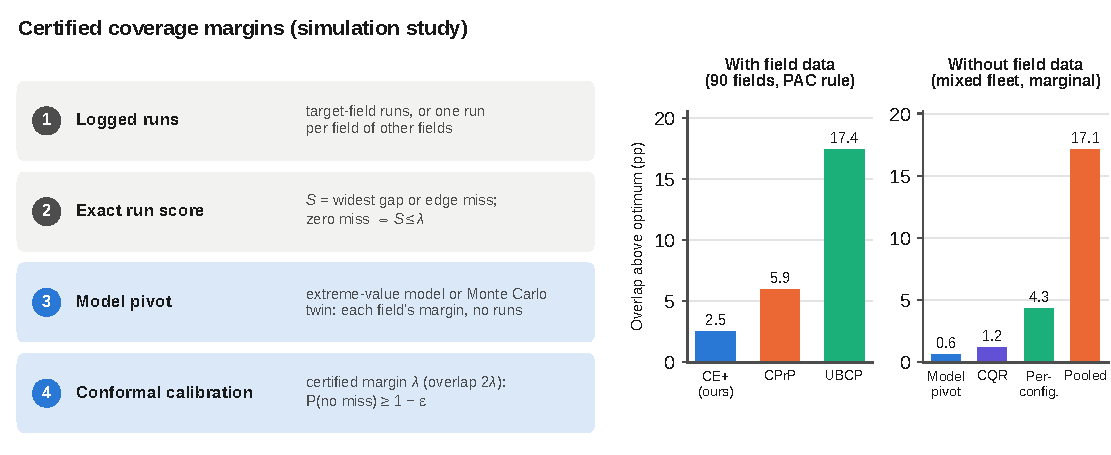
\includegraphics[width=\textwidth]{../../../figures/paper/graphical_abstract.pdf}
\end{graphicalabstract}

\begin{highlights}
\item No missed strip reduces exactly to one score: the covering radius of passes
\item Conformal calibration certifies the miss probability of a coverage plan
\item A vehicle-model pivot certifies fields without history in mixed fleets
\item Simulation study: valid in pre-registered tests, tighter than conformal planners
\item Zero-miss margins pay off only if a miss costs 30--100x the overlapped area
\end{highlights}

\begin{keyword}
coverage path planning \sep conformal prediction \sep GNSS guidance \sep pass-to-pass accuracy \sep overlap \sep precision agriculture
\end{keyword}
\end{frontmatter}

\section*{Nomenclature}
{\footnotesize
\begin{tabularx}{\textwidth}{@{}>{\raggedright\arraybackslash}p{0.24\textwidth}X@{}}
\toprule
\textbf{Symbol / acronym} & \textbf{Meaning} \\
\midrule
\(w\) & implement (swath) width \\
\(W\) & main area: field inset by \(2w\) (the rest is headland) \\
\(\lambda\) & margin (erosion): planned overlap between adjacent passes is \(2\lambda\) \\
\(\pi(\lambda)\), \(K(\lambda)\) & greedy plan with margin \(\lambda\) and its number of passes \\
\(J(\lambda)\) & main-area overlap ratio of \(\pi(\lambda)\) \\
\(e_k(x)\) & lateral offset of executed pass \(k\) at along-pass position \(x\) \\
\(M(\lambda,e)\) & missed (unworked) area of the main area \\
\(S\) & run score (covering radius minus \(w/2\), plus the planned margin; Lemma 1) \\
\(\lambda_\mathrm{ref}\) & margin of the reference plan on which scores are calibrated \\
\(\varepsilon\), \(\delta\) & tolerated probability of a run with a missed strip; PAC confidence parameter \\
\(k_\star\) & rank of the conformal order statistic \\
\(\lambda^\star_f\) & field \(f\)'s own requirement: the smallest margin with P(no miss) = \(1-\varepsilon\) (oracle) \\
\(\hat q_f\) & model-predicted \((1-\varepsilon)\) score quantile of field \(f\) (pivot) \\
\(\kappa\) & transfer factor from the reference plan to the deployed plan (Theorem 2) \\
\(\tau\), \(r\) & tolerated gap width; cost ratio of a missed to an over-applied unit area \\
CE, CE-q, CE+ & conformal erosion with target-field runs (Table 2) \\
XCE-T, XCE-MC & cross-field conformal erosion with an analytic or Monte Carlo model pivot \\
CPrP, UBCP & comparators: conformal predictive programming \citep{zhao2024}; union-bound conformal planning, pair level \citep{lindemann2023} \\
CPP & coverage path planning \\
BCD & boustrophedon cellular decomposition \\
LQR-I & linear-quadratic regulator with integral action \\
XTE & cross-track error reported by the autosteer \\
PAC & probably approximately correct (training-conditional) \\
pp & percentage points \\
\bottomrule
\end{tabularx}}

\section{Introduction}

Field operations such as spraying, fertilising, seeding and tillage are planned as parallel passes whose spacing equals the implement width minus an overlap. The plan is optimal only if the machine follows it exactly. Real passes deviate from the planned line because of GNSS positioning error, wheel slip on slopes and wet soil, antenna roll on side slopes, mounting offsets and the finite bandwidth of the steering controller. A strip is left unworked whenever two adjacent passes drift apart by more than their overlap, or when the outermost pass drifts away from the field boundary; the relevant quantity is the relative error between adjacent passes, which the industry calls pass-to-pass accuracy. Overlap set to absorb this error applies inputs twice on the overlapped strip. Both errors carry a cost: missed strips lose yield or leave weeds and pests untreated, and overlap wastes seed, fertiliser and pesticide \citep{fao2025,zhang2015,zhang2021}. Autonomous machines remove the operator who used to correct visible gaps by eye.

Current practice sets a fixed overlap, typically twice the vendor's pass-to-pass specification or a value learned by experience. Such a margin has no stated reliability and does not adapt to field shape, terrain, receiver grade or implement width. Coverage path planning (CPP) research has produced efficient decompositions, swath-angle optimisation and smooth headland turns \citep{galceran2013,hoffmann2024,mier2023,mier2025}, and terrain-aware planners adjust spacing to 3D geometry \citep{hameed2016}, but these planners assume perfect execution. Control research reduces tracking error \citep{lenain2006,pannocchia2003,mayne2005}, but a smaller error does not by itself state how often a strip will be missed. Conformal prediction gives finite-sample, distribution-free guarantees and has been used for planning \citep{lindemann2023,zhao2024}, but three features of field coverage are not addressed: the guarantee must hold for a maximum over many pass pairs and field edges; the plan that is calibrated and the plan that is deployed differ, and adding passes makes the maximum larger; and a field is worked only a few times per year, while a conformal quantile at a miss level of 10\% needs at least 9 (marginal) or 22 (training-conditional, PAC) logged runs.

This paper makes four contributions, all evaluated in simulation driven by real field boundaries, elevation models and GNSS error series.

\begin{enumerate}
\def\labelenumi{\arabic{enumi}.}
\tightlist
\item
  \textbf{An exact score for complete coverage.} The event ``no strip is missed'' is reduced exactly to one number per run, the covering radius of the executed passes including the field edges, and this is the smallest score that can certify complete coverage (Section 3).
\item
  \textbf{Conformal erosion with target-field data.} Calibrating this score on a reference plan gives an assumption-free certificate for that plan (CE) and, under an explicit transfer assumption, for plans with fewer passes (CE-q, CE+) (Sections 4.1--4.2, 5.1--5.2).
\item
  \textbf{Cross-field certification of fields without history (XCE).} A farm or contractor typically holds many fields with one or two logged operations each. A model of the vehicle, terrain and GNSS that predicts each field's required margin, either an analytic extreme-value model or Monte Carlo of a digital twin, is used only to put fields on a common scale; the conformal guarantee does not depend on the model's accuracy (Sections 4.3, 5.3--5.4).
\item
  \textbf{An evaluation that states where the method helps and where it does not.} Pre-registered experiments on 30 to 135 unseen fields per experiment compare against conformal planners, practice rules, configuration-aware baselines and learned predictors; robustness to a misspecified model and to headland laps; the cost at which a certified margin pays off; and an information limit that bounds what any field-level scale can gain (Section 6).
\end{enumerate}

All confirmatory experiments were pre-registered in a time-stamped repository before they were run; failed and partially met claims are reported alongside met ones, and exploratory and post hoc analyses are labelled as such (Supplementary Table S20).

\section{Related work}

\emph{Coverage path planning.} Boustrophedon cellular decomposition (BCD) with swath-angle optimisation is the standard for agricultural fields \citep{hoffmann2024}. Fields2Cover provides an open implementation with heading search and Dubins turns \citep{mier2023}, \citet{mier2025} add continuous-curvature headland paths, and \citet{hameed2016} compute 3D-terrain-equivalent spacing. None attaches a probability to complete coverage.

\emph{Robust and model-based margins.} Tube MPC \citep{mayne2005}, Gaussian chance constraints with Rice's extreme-value correction \citep{rice1944}, Gaussian-process cautious control \citep{hewing2020}, Wasserstein distributionally robust CVaR \citep{mohajerin2018} and the scenario approach \citep{campi2008} bound tracking error by a model, a worst case or sampled constraints. Parametric models misrepresent the heavy, temporally clustered tail of RTK errors (Table~\ref{tab:1}), and worst-case sets are conservative.

\emph{Conformal prediction.} Split conformal prediction and its training-conditional (PAC) variant \citep{vovk2012}; conformal prediction under covariate shift and beyond exchangeability \citep{tibshirani2019,barber2023}; conformalized quantile regression \citep[CQR;][]{romano2019}; conformal risk control \citep{angelopoulos2024crc,angelopoulos2025ltt}; hierarchical conformal prediction with one sample per group \citep{dunn2023}; and functional conformal bands \citep{lei2015,diquigiovanni2022}, of which a sup-normalised run score is an instance. Conformal planning methods \citep{lindemann2023,zhao2024,sun2023,wang2025} do not address a decision-dependent maximum over pass pairs.

\emph{Extremes of Gaussian processes.} Kac--Rice formulas and Rice's method \citep{azais2009,piterbarg1996}; maxima of stationary processes \citep{leadbetter1983}; statistical linearisation \citep{booton1954,kazakov1956}.

\section{Problem formulation}

\textbf{Fields, plans and margins.} A field is a polygon; its \textbf{main area} \(W\) is the field inset by twice the implement width \(w\), the remainder being headland. After decomposition and choice of the working direction \(x\), a plan is a set of straight pass centrelines \(y_1<\dots<y_K\). For a \textbf{margin} (erosion) \(\lambda\ge0\) the greedy planner \(\pi(\lambda)\) places passes as if the footprint had half-width \(w/2-\lambda\), so that adjacent planned footprints overlap by \(2\lambda\); the number of passes \(K(\lambda)\) is non-decreasing in \(\lambda\) (Appendix A.2). The overlap ratio \(J(\lambda)\) is the swath area within \(W\) divided by the area of \(W\), minus one; an overlap of 8\% means that 8\% of the main area receives a double dose.

\textbf{Execution.} Pass \(k\) is driven with lateral offset \(e_k(x)\), so its footprint at section \(x\) is \([y_k+e_k(x)-w/2,\ y_k+e_k(x)+w/2]\) (Fig.~\ref{fig:1}). Offsets are random, correlated along and across passes (adjacent passes read the same GNSS error trajectory a pass duration apart), and their law depends on the plan through the terrain and time at which each pass is driven. Coverage is evaluated on 1 m sections across \(W\).

\begin{figure}[!htbp]
\centering
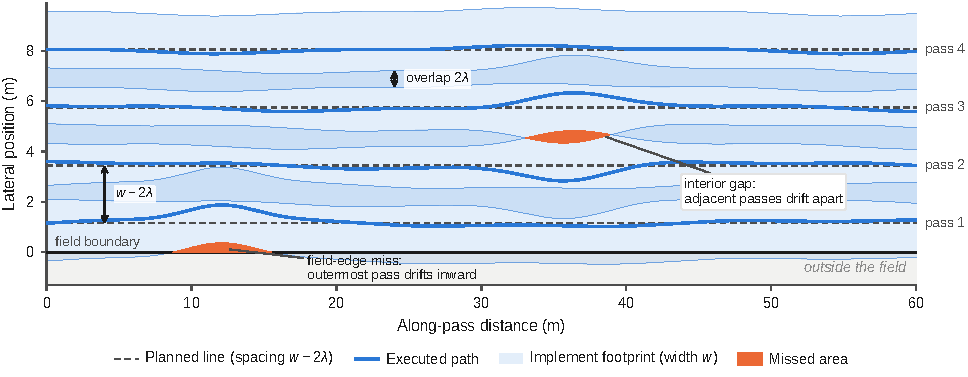
\includegraphics[width=\textwidth]{../../../figures/paper/fig_schematic.pdf}
\caption{The coverage problem. (a) One simulated run of the DGPS configuration (R3, 6 m implement) on a real paddy field, planned with that field's own 0.9 margin; the main area is inside the dashed line, and the missed strip (red, width exaggerated) is where two adjacent passes drifted apart by more than their planned overlap. (b) Detail of the framed area: planned centrelines (dashed), executed centrelines (solid) and footprint edges (dotted); the widest gap is 12 cm. (c) Cross-section at one along-pass position (schematic): footprints of width \(w\) planned at spacing \(w-2\lambda\); the chord \([\ell,u]\) is fully covered unless two executed centres are more than \(w\) apart (interior gap) or the outermost centre is more than \(w/2\) from the boundary (field-edge miss). The run score takes the worst of both over all sections (Lemma 1).}\label{fig:1}
\end{figure}

\textbf{Objective.} Let \(M(\lambda,e)\) be the missed area of \(W\) when \(\pi(\lambda)\) is executed with offsets \(e\). The certified coverage problem is
\[
\min_{\lambda}\ J(\lambda)\quad\text{s.t.}\quad \Pr\big[M(\lambda,e)=0\big]\ \ge\ 1-\varepsilon ,
\]
with \(\varepsilon\) the tolerated probability of a run with any missed strip (here 0.1). Section 4.4 generalises the event to ``no gap wider than a tolerance'' and Section 6.6 asks for which costs of a miss the zero-miss objective is worth its overlap.

\textbf{Lemma 1 (exact covering radius).} At section \(x\) let \(Y(x)\) be the executed centres of the passes relevant to the chord \([\ell(x),u(x)]\) of \(W\), sorted. The chord is fully covered iff
\[
r^\star(x)=\max\Big\{\mathrm{dist}(\ell,Y),\ \mathrm{dist}(u,Y),\ \max_{i:\ (c_i+c_{i+1})/2\in[\ell,u]}\tfrac12(c_{i+1}-c_i)\Big\}\ \le\ \tfrac w2 .
\]
For a run of the plan \(\pi(\lambda_\mathrm{ref})\) define the \textbf{run score} \(S=\lambda_\mathrm{ref}+\max_x\big(r^\star(x)-w/2\big)\). Then \(\{M=0\}\iff\{S\le\lambda_\mathrm{ref}\}\).

The score is the amount by which every footprint would have to grow (equivalently, the margin that the executed plan would have needed) to close its worst gap. Its interior terms are half the pass-to-pass gaps; the terms \(\mathrm{dist}(\ell,Y)\) and \(\mathrm{dist}(u,Y)\) are field-edge terms.

\textbf{Theorem 1 (the run score is the smallest valid score).} Call a run score valid if it never declares a run with a missed strip miss-free when the executed footprints are grown by the score (a \emph{virtual} erosion of the executed plan; Appendix A.3). Then \(S\) is valid and \(S\le S'\) for every valid score \(S'\), run by run, with no assumption on the error process. Consequently any rule that takes an order statistic of calibration scores (marginal conformal, PAC conformal, the scenario approach) deploys no more passes with \(S\) than with any other valid score, such as the per-pair or per-constraint maxima used by earlier conformal planners.

\section{Method}

Table~\ref{tab:2} summarises the variants. All compute run scores of calibration runs on a \textbf{reference plan} \(\pi(\lambda_\mathrm{ref})\), take a conformal order statistic, and deploy a plan. For \(n\) calibration scores, the \textbf{marginal rule} takes the \(k_\star\)-th smallest score with \(k_\star=\lceil(n+1)(1-\varepsilon)\rceil\), which gives \(\Pr[S_\mathrm{new}\le\hat\lambda]\ge k_\star/(n+1)\ge1-\varepsilon\) on average over calibration data. The \textbf{PAC rule} takes the smallest \(k_\star\) with \(\mathrm{BinomCDF}(k_\star-1;n,1-\varepsilon)\ge1-\delta\), which gives the guarantee conditionally on the calibration data with probability at least \(1-\delta\) (here \(\delta=0.1\)). If \(k_\star>n\) the threshold is infinite and nothing is deployed. At \(\varepsilon=\delta=0.1\) the marginal rule needs \(n\ge9\) runs and the PAC rule \(n\ge22\).

\begin{table}[!htbp]
\centering
\footnotesize
\caption{Method variants. In the pre-registrations XCE-T is called CE-EVT-R.}\label{tab:2}
\begin{adjustbox}{max width=\textwidth}
\begin{tabular}{@{}l>{\raggedright\arraybackslash}p{20.8em}>{\raggedright\arraybackslash}p{20.8em}>{\raggedright\arraybackslash}p{13.0em}>{\raggedright\arraybackslash}p{20.8em}@{}}
\toprule
\textbf{Variant} & \textbf{Calibration data} & \textbf{Score scale} & \textbf{Deployed plan} & \textbf{Guarantee on the deployed plan} \\
\midrule
CE & runs on the target field (pilot + certificate batch) & none & the reference plan itself & assumption-free (Appendix A.4) \\
CE-q & \(n\) runs on the target field & none & \(\pi(\hat\lambda)\), \(\hat\lambda\le\lambda_\mathrm{ref}\) & under the transfer assumption (S), factor \(\kappa\) (Theorem 2) \\
CE+ & \(n\) runs on the target field + 5 training fields & probe-line XTE, gated & \(\pi(t\,\sigma(z))\) & as CE-q; requires \(t\sigma(z)\le\lambda_\mathrm{ref}\) \\
XCE-T / XCE-MC & one run on each of \(n\) other fields, none on the target & model-predicted quantile (theory / Monte Carlo twin) & \(\pi(\hat q_g v^\star)\) & score guarantee assumption-free; plan via (S) \\
\bottomrule
\end{tabular}
\end{adjustbox}
\end{table}

\subsection{CE: target-field calibration, assumption-free}

CE iterates pilot batches, \(\lambda_\mathrm{ref}\leftarrow1.10\,q\) with \(q\) the \((1-\varepsilon)\) empirical quantile of pilot scores at \(\pi(\lambda_\mathrm{ref})\), until \(q\le\lambda_\mathrm{ref}\), freezes the plan, draws a fresh certificate batch, and deploys \(\pi(\lambda_\mathrm{ref})\) itself if the certificate quantile \(q^\star\le\lambda_\mathrm{ref}\) (refusing otherwise). By Lemma 1 the deployed plan is miss-free iff its score is at most \(\lambda_\mathrm{ref}\), so no transfer assumption is needed: the marginal rule bounds \(P(\text{deploy and miss})\) by \(\varepsilon\), and the PAC rule bounds the miss probability given deployment.

\subsection{CE-q and CE+: deploying fewer passes}

CE-q deploys \(\pi(q^\star)\), which has no more passes than the reference plan; its guarantee transfers from the reference plan under the coupling assumption of Theorem 2. CE+ fixes the budget at \(n\) runs and adds two elements. (1) The reference margin comes from training fields only: \(\lambda_\mathrm{ref}=1.25\times\) the largest \((1-\varepsilon)\) score quantile over five training fields. (2) Before the infield passes the machine drives one headland probe line; the autosteer's cross-track-error (XTE) RMS \(z\) is a noisy reading of the day's roughness and slip. The normalised score is \(\tilde S=S/\sigma(z)\) with \(\sigma(z)=\max(a+bz,\ 0.3\,\bar\sigma)\), \((a,b)\) fitted on training fields after dividing each field's scores by its median (\(\bar\sigma\) is the mean fitted scale), and a new operation deploys \(\lambda=t\,\sigma(z_\mathrm{new})\) with \(t\) the conformal quantile of the calibration \(\tilde S_i\). The adaptive \(\sigma\) is used only if it lowers the mean margin by at least 3\% in leave-one-field-out cross-validation on the training fields; otherwise \(\sigma\) is constant and CE+ equals CE-q with a training-field reference plan. \textbf{Transfer check (revision).} Because the transfer argument needs the deployed plan to have no more passes than the reference plan, CE+ must refuse when \(t\,\sigma(z_\mathrm{new})>\lambda_\mathrm{ref}\) and fall back to CE; the pre-registered runs did not include this check, and Section 6.3 reports how often it would have triggered.

\subsection{XCE: certifying a field without history}

A farm or contractor typically holds many fields with one or two logged operations each, and the new field has none. XCE calibrates across fields. For each field \(f\) a \textbf{model pivot} \(\hat q_f\) predicts the \((1-\varepsilon)\) quantile of the run score on the field's reference plan from controller settings, the terrain model and the GNSS grade, \textbf{without run data}. For calibration field \(f_i\) with one logged score \(S_i\), the ratio \(V_i=S_i/\hat q_{f_i}\) is formed, \(v^\star\) is the marginal or PAC order statistic of \(\{V_i\}\), and the new field \(g\) receives \(\lambda_g=\hat q_g\,v^\star\). A field whose prediction fails (\(\hat q_f\) not finite) gets \(V_f=+\infty\); if this happens on the target field, nothing is deployed.

\textbf{The guarantee does not depend on the model.} \(\hat q_f\) is a fixed function of field \(f\), independent of all run data. If fields are exchangeable and each contributes one run, the \(V\)'s are exchangeable and the conformal guarantee holds for the score (Proposition 3). Model error affects only efficiency: the closer \(V\) is to identically distributed across fields, the closer \(\lambda_g\) is to field \(g\)'s own requirement. Any field-measurable scale gives a valid method of the same form; we compare the model pivot with raw pooling (\(\hat q\equiv1\)), per-configuration pooling (Mondrian conformal), a vendor-specification scale, a learned scale \citep[CQR-type ridge regression;][]{romano2019} and an empirical per-configuration scale.

\textbf{Two implementations of the model pivot.} \emph{XCE-T} uses the analytic extreme-value model of Section 5.3; \emph{XCE-MC} uses the 0.9 quantile of 1000 Monte Carlo runs of the nominal closed-loop simulator (a digital twin) on the reference plan. Both need the same inputs; neither uses logged runs. The ratio form was chosen over a probability-integral-transform pivot, which failed in the first zero-data experiment because it amplifies errors in the far tail of the predicted distribution (Appendix B.4).

\subsection{\texorpdfstring{Tolerated gap width and the choice of \(\varepsilon\)}{Tolerated gap width and the choice of \textbackslash varepsilon}}

Many operations tolerate a narrow unworked strip (spread-pattern overlap of fertiliser spreaders, boom-end taper of sprayers). The certified event generalises to ``no gap wider than \(\tau\)'': an interior gap has width \(2(r^\star-w/2)\) and an edge strip \(r^\star-w/2\), so the score \(S_\tau=S-\tau/2\) is valid for this event (conservative for edge strips), and the certified margin is \(\hat\lambda-\tau/2\). The level \(\varepsilon\) itself is an economic choice: Section 6.6 compares the expected cost of certified and practice margins as a function of the ratio \(r\) of the cost of a missed unit area to the cost of an over-applied unit area.

\subsection{Computational cost}

CE and CE+ add only the score evaluation (a sort of executed centres per 1 m section) and an order statistic to a standard planner. The model pivot is computed once per field and reference plan, offline: XCE-T took 133--187 s per field in R1, 287--353 s in R2 and 16--51 s in R3 on one core (three fields per regime; Table S21), and XCE-MC with 1000 runs a median of 8--21 s (wall time on a shared four-core machine).

\section{Theory}

This section states what is guaranteed and under which assumptions, and describes the extreme-value model in words. Formal statements and proofs are in Appendix A, which also lists the status of every result (theorem, bound, or heuristic remark).

\subsection{Which plan is calibrated matters}

\emph{In practice: calibrate on a plan with at least as many passes as the plan you will deploy.} The run score is a maximum over pass pairs and field edges. A plan with more passes has more terms in the maximum and a stochastically larger score.

\textbf{Proposition 1 (nominal-plan calibration does not transfer).} A method that calibrates on the nominal plan \(\pi(0)\) and deploys \(\pi(\hat\lambda)\) with more passes has no distribution-free guarantee on the deployed plan: with \(K_0\) and \(K_1>K_0\) i.i.d. pair scores, a threshold calibrated at level \(1-\varepsilon\) on \(\pi(0)\) gives coverage \((1-\varepsilon)^{K_1/K_0}<1-\varepsilon\) on \(\pi(\hat\lambda)\).

The conformal planners of \citet{lindemann2023} and \citet{zhao2024}, applied to coverage, calibrate on the nominal plan. CE and its variants calibrate on a reference plan with \(\lambda_\mathrm{ref}\ge\hat\lambda\), which gives the right direction.

\subsection{Transfer from the reference plan to the deployed plan}

\emph{In practice: deploying a plan with fewer passes than the reference plan costs at most a factor \(\kappa\) on the miss level; on flat fields \(\kappa\approx1\).}

\textbf{Theorem 2 (transfer under superposition).} Couple the reference plan \(\pi_0\) and the deployed plan \(\pi_1\) by sharing the operating condition and the per-pass noise, and assume (S): for coupled runs, each matched gap or edge term of \(\pi_1\) exceeds that of \(\pi_0\) by at most \(\bar\Delta\), a bound that does not depend on the noise. Then, for every threshold \(t\),
\[
1-F_{\pi_1}(t)\le 1-F_{\pi_0}(t-\bar\Delta)=\kappa(t)\,\big(1-F_{\pi_0}(t)\big),
\]
and deploying \(\pi(\hat\lambda)\) with \(\hat\lambda\le\lambda_\mathrm{ref}\) gives \(P(\text{miss})\le\sup_{t\le\lambda_\mathrm{ref}}\kappa(t)\,\varepsilon\) (marginal rule), or \(\kappa(\hat\lambda)\,\varepsilon\) conditionally on calibration with probability at least \(1-\delta\) (PAC rule).

\begin{enumerate}
\def\labelenumi{(\Alph{enumi})}
\setcounter{enumi}{18}
\tightlist
\item
  holds exactly for a linear closed loop, because the response to the plan-dependent deterministic inputs (terrain, timing of the GNSS error) superposes on the response to the noise, and approximately for the nonlinear simulator. \(\bar\Delta\) is dominated by the roll-induced antenna offset, which differs between the passes of the two plans when the cross-slope does, plus a GNSS timing term; on flat fields \(\bar\Delta\approx0\). In the development checks, the coverage after a plan change was predicted as 0.901, 0.890 and 0.920 against simulated 0.899, 0.885 and 0.922 (Table S5). A weaker, model-free version with a hazard-rate constant is given in Appendix A.7.
\end{enumerate}

\subsection{Validity of cross-field calibration}

\textbf{Proposition 3 (XCE validity).} If fields are exchangeable (i.i.d. for the PAC statement), each calibration field contributes one run at its reference plan, and \(\hat q_f\in(0,\infty]\) depends only on field \(f\), then \(\Pr[S_\mathrm{new}\le\hat q_g v^\star]\ge k_\star/(n+1)\ge1-\varepsilon\) for the marginal rule, and the PAC rule gives the conditional statement. The zero-miss guarantee for the deployed plan follows by Theorem 2.

\emph{Proof.} \(S_\mathrm{new}\le\hat q_gv^\star\iff V_\mathrm{new}\le v^\star\); apply the split-conformal lemma to the exchangeable \(V\). \(\square\)

This is the two-level setting of \citet{dunn2023} with one sample per group. The guarantee averages over which fields calibrate and over the outcome of each calibration field's single run. Given a fixed set of logged runs, the coverage averaged over new fields is a draw from \(\mathrm{Beta}(k_\star,n+1-k_\star)\): at \(n=29\) and \(k_\star=27\) its standard deviation is about 0.054, so one realised coverage can fall well below \(1-\varepsilon\) without contradicting the guarantee. The guarantee is also an average over fields, not a per-field or per-machine statement; Section 6.4 reports coverage per machine configuration.

\subsection{A model of the required margin}

The model pivot of XCE needs a prediction of each field's \((1-\varepsilon)\) score quantile from quantities known before any operation: the controller and its gains, the terrain model of the field, the soil-moisture range, the GNSS receiver grade (through an error series of that grade) and the implement width. The analytic model chains five steps (Appendix B):

\begin{enumerate}
\def\labelenumi{\arabic{enumi}.}
\tightlist
\item
  \textbf{Closed-loop covariance.} Linearised along the noise-free closed-loop path of each pass, with describing functions for steering saturation and rate limits and a leaky-integrator model of the anti-windup clamp, the offset of one pass is a Gaussian process given the run's operating condition (soil moisture, slip and roughness gains, roll compensation, mounting bias, GNSS error trajectory); its covariance follows from a time-varying Lyapunov recursion.
\item
  \textbf{Exceedance of one pass pair and of the field edges.} The probability that a gap between two passes exceeds a threshold anywhere along the pass is bounded by a discrete Kac--Rice upcrossing sum, and computed exactly by Gaussian Monte Carlo where that bound is loose. For a field edge, the edge is missed only if every pass that covers it has receded; given the operating condition these are independent, so the edge exceedance is bounded by a product of single-pass probabilities (Appendix A.12).
\item
  \textbf{Combination over pairs.} Given the condition, non-adjacent pairs are independent, and the probability of no exceedance is approximated by the product over pairs. A Bonferroni sandwich bounds the error, but at the 0.9 level that bound is of the same size as \(\varepsilon\); the product form is accurate empirically (0.888, 0.882 and 0.900 against a true 0.900; Table S5), not by the bound.
\item
  \textbf{Mixture over operating conditions}, by sampling 200 conditions.
\item
  \textbf{Scale law.} For a stationary pair process the extremes are Gumbel, and the required margin grows like \(\sqrt{2\log L}\) in the effective length \(L\); this is a heuristic guide \citep[a tenfold larger field raises the margin by about 11\%; normal extremes converge slowly,][]{hall1979}, used only for a comparator pivot.
\end{enumerate}

The model rests on the simulator's own structure (it calls the noise-free simulator for the mean path and samples the simulator's operating conditions), as does the Monte Carlo twin; Sections 6.2 and 6.5 discuss what this implies.

\textbf{Physical reading of the edge terms.} An interior gap \((e_{k+1}-e_k)/2\) is a difference of two passes, so error shared by adjacent passes cancels in it, and its standard deviation is \(1/\sqrt2\) of that of one pass when the passes are independent. An edge term takes the full error of one pass. Edge terms therefore carry about \(\sqrt2\) times the spread of interior terms even without shared error, and more when adjacent passes share part of the GNSS error (in the 1 Hz DGPS series, the correlation at the 13--113 s between adjacent passes at one section is 0.91--0.41; for RTK 0.71--0.54). They are needed for an unbiased prediction under DGPS, but in the simulations they were the binding term of a run in only about 1\% (RTK) and 10\% (DGPS) of runs, and with headland laps that overlap the main area in 0.1\% and 1.9\% (Section 6.5).

\subsection{Margin inflation under the ideal scale}

\textbf{Proposition 4.} Let \(G_f\) be the score distribution on field \(f\), \(\lambda^\star_f=G_f^{-1}(1-\varepsilon)\) the field's own requirement, and take the ideal (unavailable) pivot \(\hat q_f=\lambda^\star_f\). With \(H(v)=\mathbb E_f[G_f(v\lambda^\star_f)]\), every new field receives \(\lambda_g/\lambda^\star_g=H^{-1}(B)\) with \(B\sim\mathrm{Beta}(k_\star,n+1-k_\star)\).

For the PAC rule with \(n=29\), \(k_\star=n\) and \(\mathbb E B=29/30\); if normalised shapes coincide, the inflation is a within-field tail ratio that the ideal pivot cannot remove. This is an identity for the ideal pivot, not a lower bound over all pivots: another pivot changes \(H\), and in one cell raw pooling was cheaper than the ideal pivot (Section 6.4). Both decisive quantities, the between-field spread relative to the model error and the within-field tail ratio, can be computed from the model before any experiment.

\section{Simulation experiments}

\subsection{Data, simulator, machine configurations and protocol}

\textbf{Data.} All inputs are public. Field boundaries and working directions come from 250 combine-harvester GNSS trajectories of the field--road trajectory dataset of the national agricultural machinery operation platform of China \citep{wu2023}; density-based clustering extracts 964 fields, of which 137 paddy fields (hilly south of China) and 162 wheat fields (North China Plain) are used. Terrain comes from Copernicus GLO-30 elevation windows \citep{esa2021}. GNSS error comes from 12 NOAA CORS station pairs (baselines 5--30 km, in agricultural regions of the US Midwest and Great Plains), 8 days each across four seasons of 2024--2025, processed with RTKLIB \citep{takasu2009} in its demo5 fork \citep{everett_demo5} as a moving rover against the reference coordinates at four receiver grades (Table~\ref{tab:1}). The 30 s epochs are interpolated to 1 Hz and high-frequency residuals of a vehicle GNSS/INS record \citep{tang2022} are added. Each simulated run draws a station-pair-day and a start time.

\begin{table}[!htbp]
\centering
\footnotesize
\caption{Horizontal error of the processed CORS series (96 station-pair-days per grade, 30 s epochs, first 30 min of each day removed). The RTK tail comes from wrong fixes and float drift lasting minutes; a Gaussian with the same RMS underestimates it by orders of magnitude. Static geodetic antennas lack vehicle multipath, canopy masking and correction-link outages, and the stations are in the US while the fields are in China; Section 6.5 therefore also tests a degraded-GNSS variant.}\label{tab:1}
\begin{adjustbox}{max width=\textwidth}
\begin{tabular}{@{}l>{\raggedright\arraybackslash}p{20.8em}llll@{}}
\toprule
\textbf{Grade} & \textbf{Processing} & \textbf{RMS} & \textbf{95\%} & \textbf{99.9\%} & \textbf{Max} \\
\midrule
RTK & carrier phase, continuous ambiguity resolution (84\% of epochs fixed, 16\% float) & 2.4 cm & 3.3 cm & 24.5 cm & 1.39 m \\
RTK float & carrier phase, no ambiguity resolution & 2.6 cm & 4.0 cm & 24.6 cm & 1.39 m \\
DGPS & code differential & 32.5 cm & 57.8 cm & 2.05 m & 6.05 m \\
Single point & L1 code & 1.51 m & 2.78 m & 4.97 m & 7.16 m \\
\bottomrule
\end{tabular}
\end{adjustbox}
\end{table}

\textbf{Simulator.} A closed-loop simulator (time step 0.05 s, speed 2 m/s) integrates kinematic steering with a first-order steering lag of 0.25 s, 35° saturation and a 30°/s rate limit; terrain slip proportional to the lateral gradient plus Ornstein--Uhlenbeck roughness, both scaled by per-run soil moisture; a 2.6 m antenna with roll compensation \(0.85\pm0.05\); a per-run mounting bias (standard deviation 1.5 cm); and GNSS error projected on the lateral axis. Passes are executed in real time order with headland turns, so adjacent passes read the same error series one pass duration apart. The default controller is LQR with integral action (LQR-I); pure pursuit, Stanley, a slip observer \citep{lenain2006} and offset-free MPC \citep{pannocchia2003} are alternatives. The footprint is centred on the vehicle reference point (a rigidly mounted implement); Section 6.5 tests a trailed implement. Details are in Appendix C.

\begin{table}[!htbp]
\centering
\footnotesize
\caption{Machine configurations (one implement width, GNSS grade and controller each). The mixed fleet of Section 6.4 pools all three. Paddy slopes come from the 30 m elevation model, which does not resolve levelled basins; Section 6.5 tests levelled terrain.}\label{tab:3}
\begin{adjustbox}{max width=\textwidth}
\begin{tabular}{@{}lllll>{\raggedright\arraybackslash}p{7.3em}@{}}
\toprule
\textbf{Configuration} & \textbf{Fields} & \textbf{GNSS grade} & \textbf{Width \(w\)} & \textbf{Soil moisture} & \textbf{Vendor pass-to-pass} \\
\midrule
R1 RTK, flat, 3 m & wheat (plain) & RTK & 3 m & Beta(2, 3) & 2.5 cm \\
R2 RTK, hilly-wet, 1.5 m & paddy (hilly) & RTK & 1.5 m & 0.6--0.9 & 2.5 cm \\
R3 DGPS, hilly, 6 m & paddy (hilly) & DGPS & 6 m & Beta(2, 3) & 20 cm \\
\bottomrule
\end{tabular}
\end{adjustbox}
\end{table}

\textbf{Metrics.}

\begin{itemize}
\tightlist
\item
  \emph{P(no miss)}: fraction of test runs with zero missed area, pooled over fields (the run-level coverage).
\item
  \emph{Meet rate}: fraction of fields whose P(no miss) over 200 test runs is not significantly below 0.9 (one-sided binomial test at 0.05; a correctly calibrated marginal method meets it on about 85\% of fields, a PAC method on about 99\%; Appendix A.19).
\item
  \emph{Overlap}: main-area overlap ratio \(J\) of the deployed plan; \emph{applied overlap} additionally counts swath reaching into the headland.
\item
  \emph{Missed area}: mean fraction of the main area left unworked.
\item
  \emph{Regret / excess overlap}: overlap minus that of the field's \textbf{oracle} plan, the smallest margin whose own P(no miss) is 0.9 on test-distribution runs, in percentage points (pp). The oracle uses test runs and is a reference point, not an attainable method: a method can fall below it on a field by chance.
\end{itemize}

\textbf{Experiments.} Fields are ordered once with a fixed seed and split by index so that each confirmatory experiment uses fields not used by the analyses that designed it (Appendix C.2). The experiments, with their repository names, are:

\begin{itemize}
\tightlist
\item
  \emph{Experiment A, fields with operation history}: A1, a pre-registered comparison on 90 fresh fields (repository ``v8''); A2, calibration with few runs (revision, pre-registered).
\item
  \emph{Experiment B, fields without history}: B1--B3, three pre-registered zero-data experiments (``E-low v1--v3''); B4, a pre-registered check of the guarantee over random field splits and redrawn logged runs; B5, configuration-aware baselines and per-configuration coverage (revision, pre-registered).
\item
  \emph{Experiment C, robustness}: C1, model mismatch; C2, headland laps (revision, pre-registered).
\item
  \emph{Cost analysis} (descriptive).
\end{itemize}

Pre-registrations were committed before the corresponding computations (Supplementary Table S20 lists the status of every result). All registered zero-data experiments used the extreme-value model without the field-edge terms; validity is unaffected, and Section 6.2 reports what the edge terms change.

\subsection{How accurate is the model pivot?}

Fig.~\ref{fig:2} compares the predicted 0.9 quantile of the run score on each field's reference plan with the empirical 0.9 quantile of 200 independent simulated runs, on the 45 test fields of each configuration. The 200-run reference quantile is itself noisy; the Monte Carlo twin with 1000 fresh runs differs from it by a log standard deviation of 0.030 (R1), 0.032 (R2) and 0.083 (R3), which is essentially this sampling noise. The analytic model differs from it by 0.039, 0.038 and 0.107, with mean bias +1.0\%, +0.1\% and +0.9\%; its own error, net of the reference noise, is therefore about 2--3\% under RTK. Under DGPS, the model without field-edge terms was biased low (−5.2\%, log standard deviation 0.097, on the same 45 fields). The edge terms (Theorem A2(b), Appendix A.12) were derived after this observation on 15 fields and then computed, unchanged, on the remaining 30 (revision, pre-registered as a descriptive check): on these 30 they moved the bias from −5.7\% to +0.9\% but widened the scatter from 0.089 to 0.106 (Appendix B.3), so they correct the level of the DGPS margins, not their field-to-field ranking. The analytic model needs 16--353 s per field without and a median of 271 s (up to 40 min) with the edge terms, and the twin a median of 8--21 s (Table S21), all once per field and offline.

These checks verify the model against the simulator it was built from. The model calls the noise-free simulator for the mean path and samples operating conditions from the simulator's own distribution, and its refinements were introduced because earlier checks against the same simulator failed (Appendix B.1). Fig.~\ref{fig:2} therefore shows internal consistency, not realism; Section 6.5 asks what happens when the simulated reality differs from the model.

\begin{figure}[!htbp]
\centering
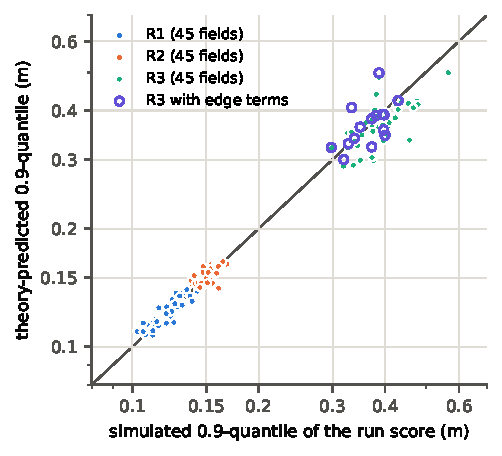
\includegraphics[width=\textwidth]{../../../figures/paper/fig_theory_vs_sim.pdf}
\caption{Predicted versus simulated 0.9 quantile of the run score (m, log--log), one point per field, 45 fields per configuration. (a) Analytic extreme-value model (R3 with field-edge terms); (b) Monte Carlo twin (1000 runs of the nominal simulator). The simulated value is the empirical 0.9 quantile of 200 independent runs; the shaded band is ±10\%.}\label{fig:2}
\end{figure}

\subsection{Experiment A: fields with operation history}

\textbf{A1, pre-registered comparison on 90 fresh fields.} The registration fixed two claims on fields 50--79 of each configuration: \textbf{V} (validity), CE+ pooled P(no miss) not significantly below 0.9 and CE+ PAC failing the meet test on fewer than 9 of 30 fields; \textbf{E} (efficiency within the guarantee class), CE+ has lower main-area overlap than conformal predictive programming \citep[CPrP;][]{zhao2024} and union-bound conformal planning at pair level \citep[UBCP;][]{lindemann2023}, in both classes, by one-sided paired Wilcoxon tests with Holm correction over 12 comparisons. All methods used 100 calibration runs per field and the BCD + LQR-I stack. Both claims were met in every configuration (Table~\ref{tab:4}). Table~\ref{tab:4} also shows the two practice rules, which the registration did not include as comparators.

\begin{table}[!htbp]
\centering
\footnotesize
\caption{Experiment A1 (pre-registered; 30 fresh fields per configuration). Overlap reductions of CE+ against CPrP and UBCP, within the guarantee class: 18.9\% and 22.7\% (R1 marginal), 21.2\% and 34.3\% (R1 PAC), 4.1\% and 9.7\% (R2 marginal), 4.0\% and 37.2\% (R2 PAC), 23.8\% and 35.1\% (R3 marginal), 25.5\% and 54.7\% (R3 PAC); all 12 Holm-significant (largest Holm p 0.0225). CE+ marginal is not significantly below 0.9 (field-clustered p 0.70, 0.98, 0.29); CE+ PAC fails the meet test on 0 of 30 fields in every configuration. Practice rules, missed area and regret are descriptive. The vendor rule is twice the nominal pass-to-pass accuracy; the farmer-tuned margin was tuned once on the five training fields.}\label{tab:4}
\begin{adjustbox}{max width=\textwidth}
\begin{tabular}{@{}l>{\raggedright\arraybackslash}p{13.0em}lllll@{}}
\toprule
\textbf{Config.} & \textbf{Method} & \textbf{P(no miss)} & \textbf{Meet rate} & \textbf{Missed area \%} & \textbf{Overlap \%} & \textbf{Regret pp} \\
\midrule
R1 & CE+ / CE+ PAC & 0.903 / 0.941 & 0.93 / 1.00 & 0.001 / 0.001 & \textbf{8.39} / \textbf{9.04} & −0.26 / +0.38 \\
\textasciitilde{} & CPrP / CPrP PAC & 0.944 / 0.967 & 1.00 / 1.00 & 0.001 / 0.000 & 10.35 / 11.47 & +1.69 / +2.82 \\
\textasciitilde{} & UBCP / UBCP PAC & 0.959 / 0.988 & 1.00 / 1.00 & 0.001 / 0.000 & 10.86 / 13.76 & +2.20 / +5.10 \\
\textasciitilde{} & Vendor rule; farmer-tuned & 0.000; 0.897 & 0.00; 0.70 & 0.216; 0.001 & 1.75; 9.22 & −6.90; +0.57 \\
R2 & CE+ / CE+ PAC & 0.911 / 0.944 & 0.90 / 1.00 & 0.001 / 0.001 & \textbf{25.62} / \textbf{28.14} & +0.70 / +3.22 \\
\textasciitilde{} & CPrP / CPrP PAC & 0.923 / 0.956 & 0.97 / 1.00 & 0.001 / 0.001 & 26.72 / 29.32 & +1.80 / +4.40 \\
\textasciitilde{} & UBCP / UBCP PAC & 0.944 / 0.991 & 0.97 / 1.00 & 0.001 / 0.000 & 28.38 / 44.80 & +3.46 / +19.87 \\
\textasciitilde{} & Vendor rule; farmer-tuned & 0.000; 0.834 & 0.00; 0.20 & 0.642; 0.001 & 3.46; 23.00 & −21.46; −1.92 \\
R3 & CE+ / CE+ PAC & 0.896 / 0.933 & 0.90 / 1.00 & 0.027 / 0.020 & \textbf{15.73} / \textbf{19.30} & +0.45 / +4.02 \\
\textasciitilde{} & CPrP / CPrP PAC & 0.946 / 0.969 & 1.00 / 1.00 & 0.017 / 0.013 & 20.63 / 25.89 & +5.35 / +10.61 \\
\textasciitilde{} & UBCP / UBCP PAC & 0.960 / 0.983 & 1.00 / 1.00 & 0.014 / 0.006 & 24.22 / 42.61 & +8.94 / +27.33 \\
\textasciitilde{} & Vendor rule; farmer-tuned & 0.403; 0.834 & 0.00; 0.47 & 0.120; 0.036 & 7.59; 13.53 & −7.69; −1.75 \\
\bottomrule
\end{tabular}
\end{adjustbox}
\end{table}

\begin{figure}[!htbp]
\centering
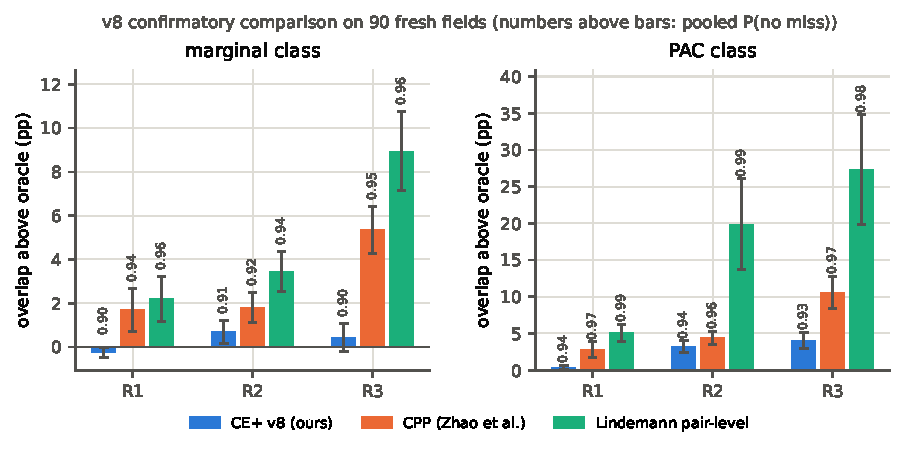
\includegraphics[width=\textwidth]{../../../figures/paper/fig_v8_regret.pdf}
\caption{Regret (overlap above the per-field oracle, pp) in Experiment A1 for the marginal (a) and PAC (b) guarantee classes; bars are means over 30 fields with 95\% intervals, and numbers above bars are pooled P(no miss).}\label{fig:3}
\end{figure}

\emph{What the gain is made of.} All compared methods deploy plans from the same family \(\pi(\lambda)\) and differ only in how \(\lambda\) is chosen, so at equal realised coverage they would deploy the same plan. The gain is calibration tightness: the comparators calibrate pair or per-constraint scores on the nominal plan or through a union bound and over-cover (P 0.92--0.99 at a nominal 0.9), which is what their extra overlap buys; CE+ reaches its target (Fig.~\ref{fig:3}). Most of the gain comes from the exact score and the reference plan, not from the probe-line normalisation: CE-q, which has neither the normalisation nor the training-field reference plan, reached 8.82\%, 25.51\% and 16.19\% overlap in R1--R3 against 10.35\%, 26.72\% and 20.63\% for CPrP. Measured as regret, CE+ was 27--95\% below the comparators in the cells where its regret is positive. The applied overlap including the headland gave the same direction in all 12 comparisons (reductions 2.8--29.3\%, all Holm-significant; Table S22).

\emph{Transfer check.} The transfer argument needs the deployed margin to be at most the reference margin. In R1 and R2 this held on every field. In R3 the mean deployed CE+ margin exceeded \(\lambda_\mathrm{ref}\) on 9 of 30 fields (marginal) and 19 of 30 (PAC); on those fields the guarantee rests on no theorem, although the measured coverage held (pooled P 0.896 and 0.933, meet rate 0.90 and 1.00). With the transfer check of Section 4.2, these fields fall back to the assumption-free CE, which in R3 deployed 17.77\% overlap at P 0.928.

\emph{Other stacks.} On six planner--controller stacks, CE and CE+ met their design meet rates except CE+ on follow-previous-pass guidance in R2 (P 0.850, meet rate 0.70), where steering each pass relative to the previous executed pass couples passes and violates the transfer assumption; the assumption-free CE met its target there (Table S23).

\emph{Practice rules.} The vendor rule (twice the nominal pass-to-pass accuracy) missed some strip on almost every run, but only 0.22\%, 0.64\% and 0.12\% of the main area. The farmer-tuned margin met the target on 70\%, 20\% and 47\% of fields, with 0.8 pp more overlap than CE+ in R1 and 2.6 and 2.2 pp less in R2 and R3. Whether CE+'s extra reliability is worth its overlap is a question of cost (Section 6.6).

\textbf{A2, few runs per field (revision, pre-registered).} A2 replaces the 100 calibration runs by \(n=9\)--100 runs drawn from 200-run banks on 45 fields per configuration (2000 replicates per field; CE-q, the variant CE+ reduces to under constant normalisation; deployed plans evaluated on independent test runs). Both registered predictions were met: marginal mean coverage was 0.896--0.943, never below 0.895, and in line with the exact value \(k_\star/(n+1)\) (0.900, 0.938, 0.913, 0.902, 0.901 for \(n=9\), 15, 22, 40, 100); the PAC fraction of replicates with coverage at least 0.9 was 0.890--0.951 against a required 0.88 (Table S24). The price of few runs is overlap. With 9 runs the marginal rule cost 1.3, 4.0 and 8.3 pp above the oracle in R1--R3; the PAC rule needs at least 22 runs and then cost 3.4, 10.0 and 18.7 pp, falling to 1.1, 3.2 and 4.3 pp with 100 runs. With fewer than about 20 logged operations per field, cross-field calibration (Experiment B) is the practical route.

\subsection{Experiment B: fields without operation history}

\textbf{B1--B3, pre-registered zero-data experiments.} Three experiments were registered in sequence, each designed from the previous one's results and run on fields that no earlier zero-data analysis had used (Table~\ref{tab:5}; details in Supplementary D.3--D.6).

\begin{table}[!htbp]
\centering
\footnotesize
\caption{The pre-registered zero-data sequence (all with the model without field-edge terms). Excess overlap is the deployed overlap minus the per-field oracle overlap.}\label{tab:5}
\begin{adjustbox}{max width=\textwidth}
\begin{tabular}{@{}l>{\raggedright\arraybackslash}p{20.8em}>{\raggedright\arraybackslash}p{20.8em}>{\raggedright\arraybackslash}p{20.8em}@{}}
\toprule
\textbf{Experiment} & \textbf{Method; test fields; \(n\)} & \textbf{Registered claims} & \textbf{Outcome} \\
\midrule
B1 & probability-integral-transform pivot; 148 fields; 30 & valid and ≥ 10\% less excess overlap than the strongest valid comparator, every configuration & \textbf{Not met} in R1--R3 (+5.35, +3.98, +5.70 pp vs +3.22, +3.26, +1.31 pp) \\
B2 & XCE-T; 90 fields; 29 & C1: R1 PAC, and C2: R3 marginal, ≥ 10\% better than raw pooling & \textbf{Both met} (Holm p 0.0002, 0.0012), but mostly through realised coverage at one calibration draw: at matched coverage all pivots of a configuration lay within 0.42 pp \\
B3 & XCE-T and a gated variant; 45 fields + mixed fleet; 25 & C3: mixed fleet, ≥ 10\% better than every comparator, both classes; C4: gated variant never worse than the best comparator & \textbf{Partly met.} C3: 5 of 8 comparisons met; C4: 1 of 6 cells \\
\bottomrule
\end{tabular}
\end{adjustbox}
\end{table}

B1 failed because the probability-integral-transform pivot amplifies tail errors (Appendix B.4). B2 met both claims, but at matched coverage all pivots of a configuration lay within a few tenths of a point, so B2 does not show that the model pivot is more efficient within one configuration. In B3, XCE-T in R1 (marginal) realised 0.877 against its registered criterion of 0.89, over subsets drawn from one fixed set of logged runs; B4 tests whether such values are draws of the calibration data.

\textbf{B4, does the guarantee hold? (pre-registered).} B4 redrew both the calibration fields (25 of 45 per configuration, or of 135 in the mixed fleet) and each calibration field's logged run (from a bank of 200 independent runs), 4000 times per scenario, pivot and rule. All 26 cells met their criteria (Table S19a, Fig. S1); the observed marginal means (0.919--0.929), marginal fractions with coverage ≥ 0.9 (0.689--0.767) and PAC fractions (0.911--0.949) agree with their exact targets of 0.923, 0.729 and 0.928. The sub-0.9 values of B2 (0.844) and B3 (0.877) are therefore draws of the calibration data. B4 cannot detect a failure of exchangeability, because it splits a fixed set of fields at random.

\textbf{B5, configuration-aware baselines and per-configuration coverage (revision, pre-registered).} The mixed fleet pools three machine configurations. The registered B3 and B4 compared the model pivot mainly with configuration-blind pooling, which a contractor would not use. B5 adds per-configuration (Mondrian) pooling, an empirical per-configuration scale, a configuration-aware learned scale (CQR, trained on separate fields) and the Monte Carlo twin, and reports coverage per configuration (Table~\ref{tab:6}, Fig.~\ref{fig:4}).

\begin{table}[!htbp]
\centering
\footnotesize
\caption{Experiment B5 (revision, pre-registered): mixed fleet of 135 fields, 4000 replicates. Overall validity held for every non-refusing pivot (marginal mean coverage 0.896--0.925; PAC fraction 0.892--0.955). Per-configuration coverage is not guaranteed by the theorem; values below 0.88 are in bold. Mondrian excess is over deployed fields; refused fields need another rule. XCE-T without field-edge terms is the registered pivot; the row with edge terms uses them on all 45 DGPS fields.}\label{tab:6}
\begin{adjustbox}{max width=\textwidth}
\begin{tabular}{@{}>{\raggedright\arraybackslash}p{14.6em}>{\raggedright\arraybackslash}p{10.9em}>{\raggedright\arraybackslash}p{16.1em}>{\raggedright\arraybackslash}p{11.4em}@{}}
\toprule
\textbf{Pivot} & \textbf{\(n=25\): coverage R1 / R2 / R3 (marginal)} & \textbf{\(n=25\) excess, marginal / PAC} & \textbf{\(n=60\) excess, marginal / PAC} \\
\midrule
Raw pooling & 0.999 / 0.998 / \textbf{0.779} & +29.19 / +63.97 & +17.12 / +37.98 \\
Spec. × scale law & 0.944 / \textbf{0.840} / 0.993 & +12.95 / +23.09 & +9.93 / +14.98 \\
Mondrian (per configuration) & 0.958 / 0.960 / 0.957 & refuses on 56\% / 100\% of fields & +4.35 / refuses on 74\% \\
Per-configuration scale & 0.939 / 0.958 / 0.842 & +4.57 / +19.94 & +1.29 / +6.42 \\
CQR (configuration-aware) & 0.961 / 0.942 / 0.866 & +4.09 / +18.86 & +1.20 / +6.19 \\
\textbf{XCE-T} (analytic model) & 0.931 / 0.936 / 0.904 & \textbf{+2.89} / +14.56 & \textbf{+0.57} / +4.37 \\
\textbf{XCE-T} with field-edge terms & 0.927 / 0.931 / 0.917 & +3.03 / \textbf{+13.69} & +0.63 / +4.36 \\
\textbf{XCE-MC} (Monte Carlo twin) & 0.924 / 0.929 / 0.913 & \textbf{+2.68} / \textbf{+13.76} & \textbf{+0.55} / \textbf{+4.19} \\
\bottomrule
\end{tabular}
\end{adjustbox}
\end{table}

All four registered predictions were met (Table~\ref{tab:6}, Fig.~\ref{fig:4}). Every non-refusing pivot was valid overall. Raw pooling covered the DGPS configuration at only 0.779 (marginal) while over-covering the RTK fields at 0.999: the overall guarantee averages over configurations and can hide a badly served one. The model pivots covered every configuration at 0.885--0.936; with the field-edge terms the DGPS fields were covered at 0.899--0.924 instead of 0.834--0.904 (Table S26), at the same excess overlap. Mondrian pooling, valid per configuration, needs at least 9 (marginal) or 22 (PAC) calibration fields per configuration; with 25 calibration fields shared by three configurations it refused on 56\% of new fields (marginal) and on all (PAC). With 60 calibration fields, the model pivots cost 0.55--0.63 pp of excess overlap (marginal) against 1.20--1.29 pp for the learned and empirical configuration-aware scales and 4.35 pp for Mondrian, and 4.2--4.4 pp (PAC) against 6.2--6.4 and 12.2 pp.~The configuration-aware scales left the DGPS fields under-covered (0.82--0.87), because a scale learned from one run per field does not capture the heavier DGPS tail. The analytic model and the Monte Carlo twin were equivalent (within 0.8 pp in every cell).

\begin{figure}[!htbp]
\centering
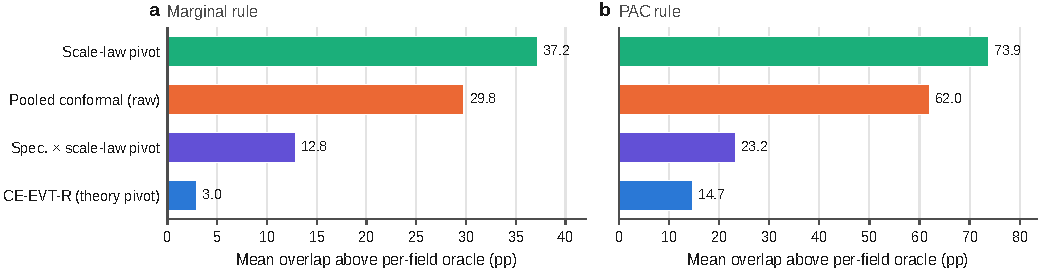
\includegraphics[width=\textwidth]{../../../figures/paper/fig_mixed_fleet.pdf}
\caption{Experiment B5: mean excess overlap of the scale pivots on the mixed fleet with 60 calibration fields (XCE-T with the field-edge terms), marginal (a) and PAC (b) rule (excess over deployed fields; a pale bar marks a pivot that refuses on part of the fields), and mean coverage of the DGPS fields under the marginal rule with 25 calibration fields (c; dashed line 0.9).}\label{fig:4}
\end{figure}

\textbf{B6, model accuracy against learned predictors (post hoc).} Trained on the one run per field that this setting provides, cross-validated ridge regression and gradient boosting on field features did not reach the model's accuracy within the available pools (standard deviation of log(prediction / \(\lambda^\star_f\)) at the largest pool: 0.070 and 0.109 vs 0.029 in R1; 0.043 and 0.049 vs 0.029 in R2; 0.148 and 0.190 vs 0.056 in R3; Table S25). A feature correction of the model with a cross-validated penalty matched the model in R2 (0.029) and did not improve on it elsewhere. Trained on oracle targets, which need hundreds of runs per field, ridge regression beat the model under RTK (0.021 in R1 and R2) but not under DGPS (0.079). The Monte Carlo twin with 1000 runs was slightly more accurate than the analytic model (0.025, 0.026, 0.047), as expected for an exact simulation of the same model.

\subsection{Experiment C: robustness}

\textbf{C1, model mismatch (revision, pre-registered).} Six ``truth'' variants change the simulated reality while the model pivots, the Monte Carlo twin and all fixed pivots keep the nominal model: T1 intermittent wet patches with heavy-tailed slip pulses; T2 a trailed implement (hitch length 5 m, downhill crab); T3 per-run speed 1.5--3.0 m/s with 0.15 s steering latency and a 0.3° deadband; T4 GNSS error 1.5 times larger; T5 terrain gradients reduced to a quarter (levelled basins); T6 the combination T1--T4. For every field and variant, 200 calibration runs and a 28-point margin curve were simulated from the truth.

Table~\ref{tab:7} shows the result. \textbf{Validity.} The score-level guarantee does not involve the model, and all pivots remained valid overall in five of six variants. In T1, which adds heavy-tailed slip pulses that roughly double the RTK margin, the overall marginal coverage of every pivot fell to 0.892--0.895 with 60 calibration fields (criterion 0.895; exact expectation 0.902), and target-field CE-q with 100 runs reached 0.893 (R1) and 0.891 (R2). The cause is the transfer step, not the conformal step: the reference margin had been set from nominal training fields, and in T1 the deployed RTK margin exceeded it on 91--100\% of fields, so the deployed plan had more passes than the calibrated one (Proposition 1). The transfer check of Section 4.2 would have refused these deployments; a reference margin set from data of the actual configuration avoids them. \textbf{Model accuracy.} Mismatch that rescales the error moderately left the model useful: with a trailed implement (bias +0.42, the implement low-pass filters the tractor's error), degraded GNSS (−0.35 under DGPS) or levelled terrain, the model pivot remained the most efficient pivot of the mixed fleet (0.5--0.7 pp against 3.8--42.7 pp for the others). Mismatch that changes the error structure did not: with wet patches the model underpredicted RTK margins by a factor of 2 (bias −0.73), and with a faster vehicle, steering latency and a deadband the DGPS loop became unstable and the model underpredicted by a factor of 2.7; in the combined variant the vendor-specification scale was more efficient than the model (8.7 vs 14.1 pp). The Monte Carlo twin, which shares the model's assumptions, failed in the same cases. \textbf{Per-configuration coverage.} Whenever the mismatch affected one configuration more than the others (T2, T3, T4, T6), the model pivot no longer equalised coverage across configurations, and the DGPS fields were covered at 0.78--0.85, better than raw pooling (0.71--0.80) but below target. None of the four registered predictions was met in every variant: P4.1 (overall validity) and P4.4 (CE-q validity) failed in T1 only, P4.2 (model log-error standard deviation below 0.15) failed in T1, T3 and T6, P4.3 (model pivot excess below half of raw pooling and below the specification scale, 25 calibration fields) held in T2, T4 and T5 only (Table S27).

\begin{table}[!htbp]
\centering
\footnotesize
\caption{Experiment C1 (revision, pre-registered). Model bias: mean log ratio of the nominal-model quantile (analytic model with edge terms) to the truth quantile, 45 fields per configuration. Coverage and excess: mixed fleet, marginal rule, 60 calibration fields, 2000 replicates; DGPS coverage is the mean over the DGPS target fields. CE-q: mean coverage over 500 replicates per field. XCE-T uses the field-edge terms. Bold: below 0.895 overall, or below 0.85 for one configuration. In T3 the DGPS configuration is under-covered and excess overlap below the oracle is not an efficiency gain. Nominal row: Experiments B5 and A2.}\label{tab:7}
\begin{adjustbox}{max width=\textwidth}
\begin{tabular}{@{}l>{\raggedright\arraybackslash}p{10.9em}>{\raggedright\arraybackslash}p{10.9em}>{\raggedright\arraybackslash}p{18.7em}>{\raggedright\arraybackslash}p{10.9em}@{}}
\toprule
\textbf{Truth} & \textbf{Model bias \(\log(\hat q/q)\), R1 / R2 / R3} & \textbf{XCE-T coverage: all / DGPS (raw pooling DGPS)} & \textbf{Excess pp: XCE-T / XCE-MC / spec. × scale / Mondrian / raw} & \textbf{CE-q (\(n=100\)) coverage R1 / R2 / R3} \\
\midrule
Nominal & +0.01 / +0.00 / +0.01 & 0.902 / 0.899 (0.718) & 0.63 / 0.55 / 9.93 / 4.35 / 17.12 & 0.896 / 0.909 / 0.898 \\
T1 wet patches & −0.73 / −0.72 / −0.02 & \textbf{0.895} / 0.984 (0.823) & 2.39 / 1.77 / 45.53 / 23.49 / 7.81 & \textbf{0.893 / 0.891} / 0.897 \\
T2 trailed implement & +0.42 / +0.43 / +0.09 & 0.903 / \textbf{0.808} (0.716) & 0.49 / 0.52 / 3.93 / 3.81 / 17.86 & 0.900 / 0.903 / 0.902 \\
T3 speed, latency & +0.00 / +0.01 / −0.99 & 0.903 / 0.853 (0.801) & (R3 under-covered) & 0.899 / 0.899 / 0.924 \\
T4 GNSS × 1.5 & −0.04 / −0.02 / −0.35 & 0.901 / \textbf{0.803} (0.711) & 0.69 / 0.75 / 7.66 / 6.99 / 42.73 & 0.896 / 0.902 / 0.897 \\
T5 levelled terrain & −0.01 / +0.01 / +0.02 & 0.902 / 0.908 (0.717) & 0.56 / 0.47 / 9.99 / 3.98 / 16.47 & 0.904 / 0.899 / 0.904 \\
T6 combined & −0.48 / −0.45 / −1.82 & 0.905 / \textbf{0.780} (0.753) & 14.09 / 12.33 / 8.71 / 51.01 / 58.34 & 0.908 / 0.899 / 0.949 \\
\bottomrule
\end{tabular}
\end{adjustbox}
\end{table}

\textbf{C2, headland laps (revision, pre-registered).} The main experiments evaluate the main-area boundary as a hard edge reached only by the outermost pass. C2 adds one headland lap along each side, planned to overlap the main area by \(\lambda\) and driven after the infield passes. Even with the hard edge, a boundary term was the binding term of a run in only 1.0\% (R1), 0.8\% (R2) and 10.0\% (R3) of runs at the reference plan; with laps these fell to 0.1\%, 0.1\% and 1.9\%. Laps left the required margin unchanged under RTK and lowered it by about 6\% under DGPS (oracle margin 0.391 → 0.366 m; main-area overlap 15.12\% → 14.01\%). Both registered predictions were met: the boundary share under DGPS fell below 50\%, and target-field calibration remained valid with laps (marginal mean coverage 0.897--0.902; PAC fraction 0.885--0.907; Table S28). The field-edge terms therefore matter for an accurate DGPS prediction under a hard edge, but they do not dominate the miss probability, and where headland laps overlap the main area they lose most of their weight.

\subsection{What a certified margin costs}

The certified event ``no strip missed with probability 0.9'' counts a 1 cm sliver like a 1 m strip. Whether it is worth its overlap depends on what a miss costs. Let \(r\) be the cost of leaving one unit of area unworked divided by the cost of over-applying one unit of area (for an input-saving operation, the value of the yield or control lost on a missed strip divided by the input cost per unit area). The expected cost of a margin, in percent of the main area, is then overlap \(+\ r\times\) missed area. Table~\ref{tab:8} and Fig.~\ref{fig:5} evaluate it on the margin curves of the 45 test fields of each configuration (nominal model, descriptive).

\begin{table}[!htbp]
\centering
\scriptsize
\caption{Expected cost (overlap \% + \(r\) × missed-area \%) of practice and certified margins (descriptive). ``Certified (ideal)'' is each field's own 0.9 margin, the target of an exactly calibrated certificate; the cost-optimal margin minimises the expected cost per field given the test distribution and is a reference, not a method.}\label{tab:8}
\begin{adjustbox}{max width=\textwidth}
\begin{tabular}{@{}lllllllll@{}}
\toprule
\textbf{Config.} & \textbf{Policy} & \textbf{P(no miss)} & \textbf{Overlap \%} & \textbf{Missed \%} & \textbf{Cost, \(r=10\)} & \textbf{\(r=30\)} & \textbf{\(r=100\)} & \textbf{\(r=300\)} \\
\midrule
R1 & vendor rule & 0.000 & 2.12 & 0.160 & 3.72 & 6.92 & 18.10 & 50.04 \\
\textasciitilde{} & farmer-tuned & 0.882 & 9.05 & 0.001 & 9.06 & 9.07 & 9.11 & 9.24 \\
\textasciitilde{} & certified, \(\varepsilon=0.1\) (ideal) & 0.900 & 8.91 & 0.001 & 8.92 & 8.93 & 8.98 & 9.11 \\
\textasciitilde{} & cost-optimal margin & 0.02--0.50 & 2.5--6.0 & \textasciitilde{} & \textbf{3.54} & \textbf{4.69} & \textbf{5.92} & \textbf{7.10} \\
R2 & vendor rule & 0.000 & 5.38 & 0.336 & 8.74 & 15.45 & 38.95 & 106.09 \\
\textasciitilde{} & farmer-tuned & 0.844 & 23.02 & 0.001 & 23.03 & 23.05 & 23.11 & 23.30 \\
\textasciitilde{} & certified, \(\varepsilon=0.1\) (ideal) & 0.900 & 24.93 & 0.001 & 24.94 & 24.95 & 24.99 & 25.11 \\
\textasciitilde{} & cost-optimal margin & 0.00--0.32 & 5.9--15.0 & \textasciitilde{} & \textbf{8.58} & \textbf{11.58} & \textbf{14.78} & \textbf{17.75} \\
R3 & vendor rule & 0.437 & 7.56 & 0.112 & 8.68 & 10.91 & 18.73 & 41.07 \\
\textasciitilde{} & farmer-tuned & 0.853 & 13.35 & 0.033 & 13.68 & 14.33 & 16.62 & 23.16 \\
\textasciitilde{} & certified, \(\varepsilon=0.1\) (ideal) & 0.900 & 15.10 & 0.026 & 15.36 & 15.88 & 17.69 & 22.87 \\
\textasciitilde{} & cost-optimal margin & 0.21--0.89 & 4.6--14.4 & \textasciitilde{} & \textbf{7.15} & \textbf{10.31} & \textbf{15.21} & \textbf{21.90} \\
\bottomrule
\end{tabular}
\end{adjustbox}
\end{table}

\begin{figure}[!htbp]
\centering
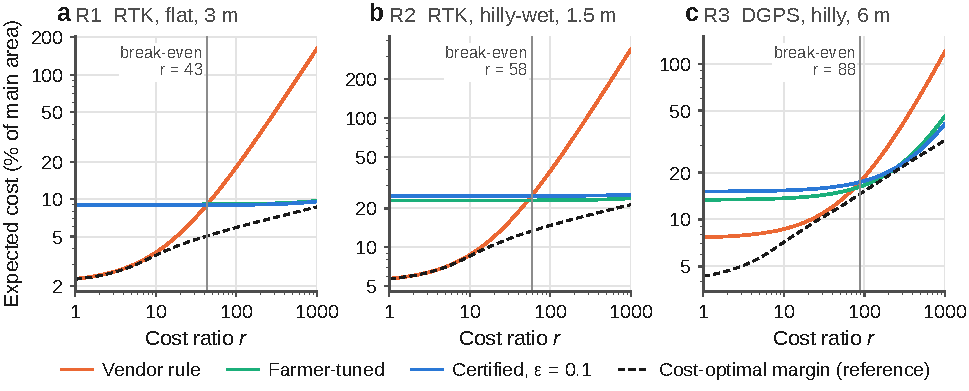
\includegraphics[width=\textwidth]{../../../figures/paper/fig_cost.pdf}
\caption{Expected cost (overlap \% + \(r\) × missed-area \%) against the cost ratio \(r\) of a missed to an over-applied unit area, for the vendor rule, the farmer-tuned margin, the certified margin at \(\varepsilon=0.1\) (each field's own 0.9 margin) and the cost-optimal margin (a reference that requires the test distribution); means over the test fields of each configuration (a--c). The vertical line marks where the certified margin becomes cheaper than the vendor rule.}\label{fig:5}
\end{figure}

Three conclusions follow. First, against the vendor rule, the certified margin pays off only above a break-even ratio of \(r^\star\approx43\) (R1), 58 (R2) and 88 (R3); with the per-operation results of Experiment A1 the break-even values are 31--35 (RTK) and 88--117 (DGPS). Second, the cost-optimal margin under RTK accepts frequent but tiny misses: even at \(r=300\) it has a P(no miss) of only 0.50 (R1) and 0.32 (R2), because RTK misses are slivers of 0.004--0.03\% of the area. Only under DGPS, whose misses are wider, does the cost-optimal margin approach the 0.9 level (\(r=300\): 0.89). Third, a tolerance helps where implements are narrow: certifying ``no gap wider than 2 cm'' instead of ``no gap'' lowers the margin by 1 cm and saves 0.9, 2.0 and 0.4 pp of overlap in R1--R3, and a 5 cm tolerance saves 2.0, 5.0 and 1.1 pp.

The value of \(r\) depends on the operation, crop and prices and is not estimated here. As an illustration only, a fertiliser strip whose omission loses a third of a crop worth five times the fertiliser cost gives \(r\approx1.7\), while a missed strip that triggers a regulatory, quarantine or resistance-management cost can give \(r\) in the hundreds. Below the break-even, a zero-miss margin at \(\varepsilon=0.1\) costs more than the vendor rule; the calibration then still states the miss probability of a cheaper margin (the same data bound \(P(S>\lambda)\) for every \(\lambda\)), and \(\varepsilon\) and \(\tau\) can be chosen by cost. Conformal risk control of the expected missed area \citep{angelopoulos2024crc} would target cost directly, but its finite-sample term \(B/(n+1)\), with \(B\) the largest possible loss, exceeds the relevant missed-area levels (0.01--0.1\%) unless thousands of runs are available.

\section{Discussion}

\subsection{What is guaranteed, and by what}

Three layers of the method rest on different assumptions. (i) The run score is exact and the smallest valid score, with no assumption (Lemma 1, Theorem 1). (ii) The conformal quantile of the score on the reference plan is distribution-free given exchangeable runs (target-field calibration) or exchangeable fields (cross-field calibration); only CE deploys that plan itself and is assumption-free. (iii) Deploying a plan with fewer passes than the reference plan (CE-q, CE+, XCE) needs the transfer assumption (S) and costs a factor \(\kappa\); the measured coverage of such plans was at or above the target whenever the deployed margin stayed below the reference margin (Experiments A2, B4, B5, C2); when it did not, coverage fell slightly below target (0.891--0.895 in the wet-patch variant of C1), which the transfer check of Section 4.2 prevents. The extreme-value model and the Monte Carlo twin affect only efficiency. The guarantee for cross-field calibration averages over fields: with configuration-blind pooling the DGPS fields of a mixed fleet were covered at 0.78 while the RTK fields were over-covered, so per-configuration coverage must be checked, and a model pivot achieved it (0.89--0.94).

\subsection{Where the method helps}

\emph{With target-field data}, the exact score and the reference plan give tight calibration: CE+ reached its target while two conformal planners over-covered at 4--55\% more overlap. The gain over well-calibrated practice is small: the farmer-tuned margin was within a few tenths of a point in R1 and below CE+ in R2 and R3, at lower reliability. \emph{Without target-field data}, a model pivot is the only configuration-aware scale that covered every configuration and was efficient: across a mixed fleet it cost 0.6 pp above the per-field optimum (marginal, 60 calibration fields) against 1.2--4.4 pp for configuration-aware baselines and 17 pp for pooling, and per-configuration pooling could not deploy at all under the PAC rule with 25 calibration fields. The analytic model and the Monte Carlo twin were equally good; the twin is simpler to build when a simulator exists, and the analytic model explains the scaling of margins with field size, the role of the field edges, and the information limit.

\subsection{Where it does not help}

Within one machine configuration, all field-level pivots, including the ideal one, perform within a few tenths of a point at matched coverage (Experiments B2--B3), because the remaining inflation is set by run-to-run randomness (Proposition 4). The PAC rule with few runs is expensive (3--19 pp above the optimum at \(n=22\)). And a zero-miss margin at \(\varepsilon=0.1\) is not cost-optimal for RTK guidance unless a missed unit costs several hundred times an over-applied one (Section 6.6); for most input-saving operations a tolerance or a larger \(\varepsilon\) is the better choice, which the same calibration supports.

\subsection{Limitations}

\begin{enumerate}
\def\labelenumi{\arabic{enumi}.}
\tightlist
\item
  \textbf{Simulation only.} Field boundaries, terrain and GNSS errors are real; execution is simulated, with a kinematic vehicle, a rigidly mounted implement in the main experiments, one speed, static US CORS errors applied to Chinese fields, and terrain slopes from a 30 m model. Experiment C1 shows that the guarantee largely survives misspecification while the model's efficiency survives only mismatch that rescales the error; heavy-tailed slip, loop instability or a combination of effects made the model pivot no better than simple scales. None of this replaces field data.
\item
  \textbf{Ground truth.} Field validation on an autonomous feed-spreading vehicle with lidar--inertial localisation is in preparation (logging and certification tools are in the repository). The run score needs the true implement position. A guidance receiver cannot see its own GNSS error, so calibration runs need an independent reference (for example a PPK rover on the implement); machine logs alone are not sufficient.
\item
  \textbf{Transfer assumption.} CE-q, CE+ and XCE deploy plans other than the reference plan and rely on (S); guidance that couples passes (follow-previous-pass) violated it.
\item
  \textbf{Exchangeability.} Cross-field calibration assumes that calibration and new fields come from one population; a new configuration or field type needs its own calibration fields. Fields worked on the same day share GNSS conditions, which the experiments did not model.
\item
  \textbf{Objective.} The zero-miss event ignores the size of a miss; Section 6.6 quantifies when this matters.
\end{enumerate}

\subsection{Practical guidance}

\begin{itemize}
\tightlist
\item
  Decide the cost ratio \(r\) of the operation first. Below a ratio of about 30--100 (RTK--DGPS in these simulations), a zero-miss margin at \(\varepsilon=0.1\) costs more than the vendor rule; use a gap tolerance \(\tau\) or a larger \(\varepsilon\), and use the calibration to state the miss probability of the margin chosen.
\item
  Record the run score (covering radius per section, including the field edges) from runs with independent ground truth; it is the tightest valid score.
\item
  Calibrate on a plan with at least as many passes as will be deployed, never on the zero-margin plan; refuse or fall back to CE if the deployed margin exceeds the reference margin.
\item
  With at least 9 (marginal) or 22 (PAC) logged operations per field, calibrate on the field (CE-q/CE+).
\item
  With many fields but one or two operations each, calibrate across fields with a model pivot, and check coverage per machine configuration; a Monte Carlo twin of the vehicle is sufficient as the model. Validate the model against a few logged runs of each configuration: where its structure is wrong (heavy-tailed slip, unstable steering), a vendor-specification scale can be as good.
\item
  Headland laps that overlap the main area remove most edge-dominated misses (Section 6.5).
\end{itemize}

\section{Conclusion}

Complete coverage of a field by a plan executed with error reduces exactly to one number per run, the covering radius of the executed passes, which is the smallest score that can certify it. Calibrated with conformal prediction on a reference plan, it gives a miss probability that is assumption-free for that plan and transfers to plans with fewer passes under an explicit coupling assumption. In simulations driven by real fields, terrain and GNSS errors, the certificate held in every pre-registered check; with target-field data it was tighter than two conformal planners, and without target-field data a model of the vehicle, terrain and GNSS, analytic or Monte Carlo, was the only scale that served every machine configuration of a mixed fleet efficiently. That advantage survived a trailed implement, degraded GNSS and levelled terrain, but not heavy-tailed slip or unstable steering, which the model does not represent; the guarantee itself fell short only when the deployed margin exceeded the calibrated one, a case the transfer check excludes. Whether a zero-miss certificate is worth its overlap is an economic question: in these simulations it pays off against the vendor rule only when a missed area costs more than about 30--100 times an over-applied one, and a gap tolerance or a larger miss level is the better choice for most input-saving operations. Field validation with independent ground truth is the next step.



\section*{Data availability}
Code, processed input data, pre-registrations (with version-control timestamps), raw results and the scripts that generate every table and figure are in the project repository, with a reproduction guide in its README; the archived version will receive a DOI on acceptance. Input data are public: the field--road trajectory dataset \citep{wu2023}, Copernicus GLO-30 \citep{esa2021}, NOAA CORS observations \citep{noaacors}, and the vehicle GNSS/INS data of \citet{tang2022}.

\section*{CRediT authorship contribution statement}
[To be completed by the authors.]

\section*{Declaration of competing interest}
The authors declare that they have no known competing financial interests or personal relationships that could have appeared to influence the work reported in this paper.

\section*{Declaration of generative AI and AI-assisted technologies in the writing process}
[To be completed by the authors according to the journal's policy.]

\section*{Acknowledgements}
[Funding sources.]

\section*{Supplementary material}
Supplementary material (proofs, theory details, experimental details and full tables) is provided in a separate file.

\bibliographystyle{elsarticle-harv}
\bibliography{refs}
\end{document}
